\section{光速不变的结论之一——运动钟的变慢}\label{sec:02.07}

现在我们来分析,从光速不变性能得出什么结论。光速不变
性使我们所看到的物理现象总是因果相继的,免除了因果倒置的
混乱。但是,光速不变性却动摇了另一个传统观念——时间间隔
的不变性。

我们可以用光速不变性来设计一种雷达钟。图\ref{fig:02.14a}~是一
个雷达式的装置,在距离雷达天线$d$处放一反射镜,那么,从天
线发出光信号到天线重又接收到这个光信号一个来回的时间间隔
应为
\begin{equation*}
  \Delta t ' = \frac { 2 d } { c }
\end{equation*}
\begin{figure}[!h]
  \centering
  \subfigure[]{
    \label{fig:02.14a}
    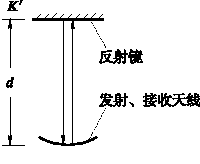
\includegraphics{figure/fig02.14a}
  }
  \quad
  \subfigure[]{
    \label{fig:02.14b}
    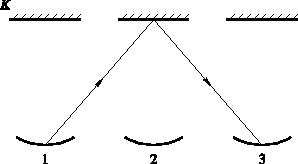
\includegraphics{figure/fig02.14b}
  }
  \caption{雷达钟}
  \label{fig:02.14}
\end{figure}

由于光速不变,我们可以用一个来回作为度量时间的单位。这个
装置就是一种钟。

现在,我们让这个钟固定在$K'$中,一起以匀速$u$相对于$K$沿
垂直于$d$的方向运动。在$K'$中看,光信号一个来回仍走$2d$,它的
时间间隔仍为
\begin{equation*}
  \Delta t ' = \frac { 2 d } { c }
\end{equation*}
% 079.jpg
但是在$K$中看来,光信号这时走的是之字形路径〔图\ref{fig:02.14b}〕。光
信号发出时,钟位于1,镜反射光信号时,位于2,接收光信号时,
位于3。因而,这光信号的一个来回,在$K$中看来是走两条斜线。
如果这个来回在$K$中看,所需时间间隔为$\Delta t$,则按光速不变性,
斜边长为$\frac { 1 } { 2 } c \Delta t $ ,底边1到2的长为$\frac { 1 } { 2 } u \Delta t$ ,故由直角三角形关系
有
\begin{align*}
  \left( \frac { 1 } { 2 } c \Delta t \right) ^ { 2 } & = \left( \frac { 1 } { 2 } u \Delta t \right) ^ { 2 } + d ^ { 2 }                                             \\
                                                      & = \left( \frac { 1 } { 2 } u \Delta t \right) ^ { 2 } + \left( \frac { 1 } { 2 } c \Delta t ' \right) ^ { 2 }
\end{align*}
解之得
\begin{equation}\label{eqn:02.07.01}
  \Delta t = \frac { \Delta t ' } { \sqrt { 1 - \dfrac { u ^ 2 } { c ^ { 2 } } } }
\end{equation}

此式表明,在$K'$中需用$\Delta t '$时间间隔的过程,在$K$中观测就
不等于$\Delta t$,而是$\Delta t > \Delta t '$ 。当$K'$中的钟走了一个单位时间间隔
即$ \Delta t ' = 1 $时,$K$中的钟已走了
$\dfrac { 1 } { \sqrt { 1 - \dfrac { u ^ 2 } { c ^ { 2 } } } } > 1$。也就是说,由$K$看
来,$K'$中的钟变慢了。$K$看$K'$的钟是在运动,故运动的钟变慢。

反过来,由$K'$来看$K$中的钟时,我们可以用完全相同的推理
方法(注意此时$K$沿$K'$的$x'$的负向以速率$u$作匀速运动),得到
\begin{equation}\label{eqn:02.07.02}
  \Delta t ' = \dfrac { \Delta t } { \sqrt { 1 - \dfrac { u ^ 2 } { c ^ { 2 } } } }
\end{equation}
可见,$K'$看$K$中的钟也变慢。

有人会说,这岂不矛盾!其实并不矛盾。因为他们是在不同
的“立场”上说话的,两种说法实际上是一致的,可以统一地表
% 080.jpg
达为: \CJKunderdot{相对于观测者运动的钟变慢}。

\clearpage
时间的变慢已有大量的实验证明。最有名的是$\mu$子的衰变。
从实验室中产生的$\mu$子,寿命只有约~$\num{2.2e-6}$~秒,这样,即使它
以光速$ c \approx \num{3e8} $米/秒运动,也只能走过
\begin{equation*}
  \num{2.2 e -6} \times \num{3e8} = 660 \text{ 米}
\end{equation*}

另一方面,宇宙射线产生$\mu$子的区域约在$1500\sim2000$米的高
空。但是我们发现不少从上层大气中产生的$\mu$子跑到地面上来了。
为什么?就因为寿命~\num{2.2 e -6}~秒是对于$\mu$子静止的参考系$K'$而
言的,当$\mu$子运动时,在地面上(即参考系$K$)看来,它的寿命应为
$\Delta t = \dfrac { \num{2.2e-6}}{ \sqrt { 1 - \dfrac { u ^ 2 } { c ^ { 2 } } } }$
秒,其中$u$是$\mu$子的运动速度,当$u$接近于$c$
时,$\Delta t$比~\num{2.2e-6}~秒大得多,即$\mu$子的寿命变长了,因而它可以
飞过距离
\begin{equation*}
  L = u \Delta t \gg 660 \text{ 米}
\end{equation*}
即能从高空飞到地面上来。

1964年,欧洲核子研究中心(CERN)通过实验定量地验证了
时间延长公式。用两个同时产生的$\mu$子,让其中之一相对于实验室
静止,另一个在加速器中运动。结果证明,运动$\mu$子的寿命变长,
两$\mu$子的寿命比值和在加速器中的运动速度$u$之间的关系完全符合
式\eqref{eqn:02.07.02}。

运动钟变慢与我们从日常生活中得来的感觉完全不同。因此,
不免有人会问:“到底钟是否真的变慢了?”物理学,特别是力
学,有很多内容是描写我们日常看到和感觉到的东西的。但是,
物理学与我们日常的直观有很多不同。物理学要求每个陈述有明
确的含义,特别是要指出每一个物理量是如何测量的,然后再在
这个基础上研究规律的建立。一般地诉诸于感觉如何如何,这不
是物理学,只不过是粗浅的认识。
% 081.jpg

\clearpage
上述的“到底”一问似乎很有道理,但却是没有物理价值的,
为什么?因为该处的“到底”是不能测量的。如果能指出“到底”
是在什么情况下进行什么测量的,我们才可作出明确的回答。如
果不能指出这一点,那说明这个问题本身就是非物理的,物理学
不研究这类问题。一旦研究测量方法,而测量又要相对于一定的
参考系,则必然走到我们上述的体系中去。

物理学的基础是测量,如果在原则上含有不能测量的东西,
这种东西本身就缺乏物理意义,因为这种不能测量的东西,既无
法用实验证实它,也无法否证它。用现代物理学的语言说,一种
理论要具有物理价值,就要具有可证伪性,即所有有关的量以及
断言,都能直接或间接由实验加以验证。这是我们判断一种理论
有没有物理价值的基本原则之一。
